\chapter{Implementierung}

Das vorliegende Kapitel widmet sich der umfassenden Dokumentation des Implementierungsprozesses des zuvor beschriebenen
Konzepts. Es bietet eine detaillierte Aufarbeitung der technischen Umsetzung und des Entwicklungsprozesses, der im
Rahmen dieser Masterarbeit durchgeführt wurde. Beginnend mit einer umfassenden Beschreibung der verwendeten Technologien
und Werkzeuge sowie einer ausführlichen Begründung für die Wahl dieser spezifischen Technologien, wird dieses Kapitel
einen tiefen Einblick in die präzise Umsetzung des Konzepts gewähren. Die Implementierung ist ein entscheidender Schritt
zur Realisierung des in den vorherigen Kapiteln skizzierten Ansatzes zur Bewertung von UML-Diagrammen. Durch die
Dokumentation dieses Schrittes wird das Verständnis für die technischen Aspekte des Projekts vertieft und ermöglicht
eine transparente Darstellung des Entwicklungsprozesses.

\section{Überblick über angewendete Werkzeuge und Technologien}
Dieses Kapitel konzentriert sich auf die Vorstellung der Werkzeuge, die für die Umsetzung des im vorherigen Kapitel
vorgestellten Konzepts verwendet werden. Es wird jedes Werkzeug vorgestellt und die Auswahl begründet.

\subsection{PlantText}

Der erste Schritt des im vorherigen Kapitel vorgestellten Konzepts besteht in der Modellierung eines UML-Diagramms.
Diese Modellierungsphase verlangt die Anwendung einer Software-Anwendung, welche in der Lage ist, das entworfene
Diagramm in ein Format zu überführen, welches für die anschließende Extraktion der enthaltenen Regelsätze dienlich
ist. Eine facettenreiche Auswahl an digitalen Werkzeugen steht zur Verfügung, um diese spezifische Aufgabe zu
bewältigen, wobei PlanText exemplarisch zu nennen ist.

PlantText~\cite{planttext} ist ein webbasiertes Instrument zur Diagrammmodellierung, das insbesondere in den Domänen
der UML und anderer Modellierungssprachen einen renommierten Status innehat. Dieses Instrument wurde entwickelt,
um die bequeme Erstellung, Bearbeitung und gemeinsame Nutzung von Diagrammen in einer kollaborativen Umgebung zu
ermöglichen. Seine Auszeichnungen resultieren aus der Benutzerfreundlichkeit, der Flexibilität und der
Leistungsfähigkeit, wodurch es zu einer favorisierten Wahl für Softwareentwickler, Systemarchitekten und Projektmanager
avanciert~\cite{planttext}.

PlantText basiert auf einer schlichten, aber wirkungsvollen Konzeption, nämlich der Generierung von Diagrammen durch
Verwendung von textuellen Notationen. Benutzer können Diagramme unter Einsatz von natürlicher Sprache und vordefinierten
Schlüsselwörtern kreieren, wodurch der gesamte Prozess simplifiziert wird. Eine prototypische Darstellung einer Klasse
in einem UML-Klassendiagramm kann etwa wie folgt aussehen:


\begin{lstlisting}[caption={[Codebeispiel] PlantText code Example}, label={lst:Planttext}, float=!ht, language=javascript]
class A {
   + attribute1: Typ1
   - attribute2: Typ2
   # operation1(): void
}
\end{lstlisting}

In diesem Illustrationsfall repräsentieren einfache Textnotationen die Klasse ``A'', ihre Attribute und Methoden.
Die Verwendung von ``+'' für öffentliche Attribute, ``-'' für private Attribute und ``#'' für Methoden gestaltet sich
intuitionsgetreu und erleichtert die Entwicklung von UML-Diagrammen erheblich. PlantText beinhaltet eine leistungsstarke
Rendering-Engine, die diese textlichen Notationen automatisiert in visuell ansprechende Diagramme konvertiert. Benutzer
sind in der Lage, die Diagramme in Echtzeit zu visualisieren und zu editieren, ohne sich mit den komplexen Details der
grafischen Gestaltung auseinandersetzen zu müssen. Diese textorientierte Herangehensweise führt zu einer höchst
effizienten und adaptierbaren Gestaltung und Veränderung von Diagrammen. Die Vorzüge der Anwendung von PlantText
manifestieren sich unter anderem in:

\begin{enumerate}
    \item \textbf{Benutzerfreundlichkeit:} PlantText ist für Einsteiger und erfahrene Modellierer gleichermaßen zugänglich.
Die Verwendung von textuellen Notationen vereinfacht den Einstieg und reduziert die Lernkurve, da sie natürlicher und
verständlicher sind als grafische Schnittstellen~\cite{mazanec2012general}.
    \item \textbf{Kollaboration und gemeinsame Nutzung:} PlantText bietet eine eingebettete Kollaborationsplattform, auf
der mehrere Benutzer simultan an Diagrammen arbeiten können. Dies fördert die Teamarbeit und erlaubt die
Echtzeit-Erstellung und Überarbeitung von Modellen~\cite{madanayake2017transforming}.
    \item \textbf{Plattformunabhängigkeit:} Da PlantText webbasiert ist, ist es plattformneutral. Benutzer können von
jedem Gerät mit Internetzugang auf ihre Modelle zugreifen und sie editieren, ohne Softwareinstallationen durchführen
zu müssen~\cite{planttext}.
    \item \textbf{Erweiterbarkeit:} PlantText unterstützt nicht ausschließlich UML, sondern auch diverse andere
Modellierungssprachen und Diagrammtypen. Infolgedessen entwickelt sich PlantText zu einem vielseitigen Werkzeug für eine
Vielzahl von Anwendungsszenarien~\cite{planttext}.
\end{enumerate}

\begin{figure}
    \centering
    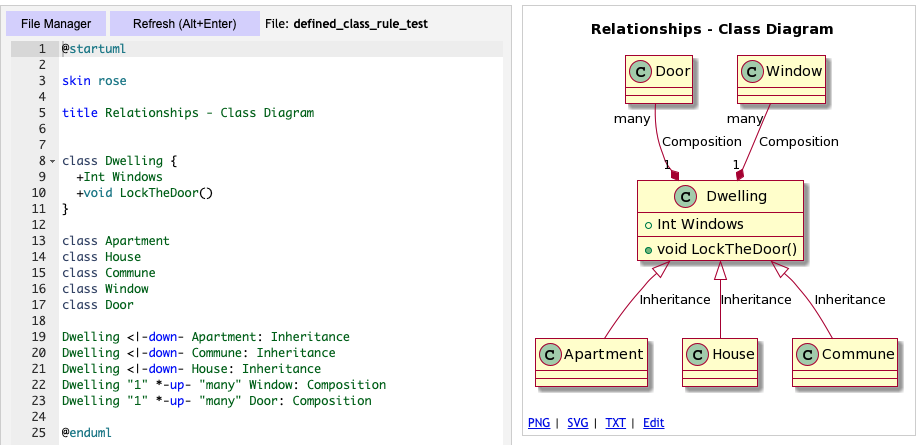
\includegraphics[width=15cm]{images/plantText}
    \caption{Grafische Benutzeroberfläche von plantText}
    \label{fig:plant-text}
\end{figure}

Vor der Wahl von PlantText als Instrument für die Entwurfsphase der Anwendung wurden mehrere Modellierungswerkzeuge
einer eingehenden Prüfung unterzogen. Diese Werkzeuge schlossen namhafte Anwendungen wie Enterprise Architect~\cite{enterarch},
Astah UML ~\cite{astah}, MagicDraw ~\cite{magic}, Visual Paradigm ~\cite{visual}, Umbrello ~\cite{umbrello} und Draw.io~\cite{draw} ein.
Eine gemeinsame Eigenschaft dieser Werkzeuge besteht darin, dass sie sich für die rasche Erstellung von Diagrammen
eignen, was auf ihre intuitive Benutzeroberfläche, leichte Verständlichkeit und Nutzerfreundlichkeit zurückzuführen ist.
Bedauerlicherweise wiesen sie jedoch einen bedeutenden Mangel auf, der ihre Anwendbarkeit in Bezug auf unsere
spezifischen Anforderungen einschränkte. Keines dieser Programme bot die Möglichkeit, die erstellten Diagramme in eine
leicht interpretierbare textuelle Form zu überführen.

Die meisten dieser Tools gestatten zwar das Exportieren der erstellten Diagramme im XML-Format, doch dieses Format
präsentiert lediglich eine räumliche Repräsentation der verschiedenen Objekte in einer Ebene, ohne eine semantische
Tiefenstruktur. Ein weiteres Hindernis bestand darin, dass die Informationen bezüglich der Verbindungen zwischen den
diversen UML-Objekten nur mit großem Aufwand und erheblichen Schwierigkeiten aus dem generierten XML extrahiert werden
konnten. Dies wäre in der Praxis äußerst zeitaufwendig und würde die Entwicklung eines eigenen Parsers erfordern, um die
relevanten Informationen zu extrahieren und in eine verwertbare Form zu überführen.

Die Nutzung von PlantText hingegen bietet einen klaren Vorteil in dieser Hinsicht. Dies resultiert aus der bereits
implementierten PlantUML-Engine, die über einen eingebauten Parser verfügt. Diese Funktionalität ermöglicht es,
den erstellten Code direkt in einem Format zu erhalten, das für die Weiterverarbeitung und Interpretation äußerst zugänglich ist.
Diese grundlegende Unterscheidung führt dazu, dass PlantText in unserem Anwendungsfall als überlegen angesehen wird.
Durch die Fähigkeit zur Bereitstellung des Modells in einer textuellen Form ermöglicht es eine tiefere und
bedeutungsvollere Analyse der erstellten Diagramme. Dies fördert die Genauigkeit bei der Modellierung und stellt sicher,
dass die erstellten Diagramme nicht nur als visuelle Darstellungen betrachtet werden, sondern auch als Quellen
semantischer Informationen dienen können.

\subsection{PlantUML Parser + Nodejs}

Im vorangegangenen Unterabschnitt wurde die Anwendung PlantText als Instrument zur Erstellung von Diagrammen
vorgestellt. Es ist jedoch essenziell zu betonen, dass PlantText lediglich die grafische Benutzeroberfläche darstellt,
da die zugrundeliegende Engine, auf der PlantText basiert, ``Plant-UML''~\cite{plantUML} ist. PlantUML ist ein Open-Source-Tool,
das von Arnaud Roques entwickelt wurde und erstmals im Jahr 2009 veröffentlicht wurde~\cite{plantUML}. Als Java-Anwendung
ermöglicht PlantUML, ähnlich wie PlantText, die Modellierung von Diagrammen, wobei die Verwendung durch die Entwicklung
von PlantText vereinfacht wurde. Alle im vorherigen Abschnitt hervorgehobenen Vorteile der Nutzung von PlantText sind in
Wirklichkeit Funktionen von PlantUML.

Eine besonders bemerkenswerte Funktion, die in diesem Abschnitt präsentiert und im Folgenden verwendet wird, ist jedoch
der PlantUML-Parser~\cite{plantUMLParser}. PlantUML ist im Wesentlichen eine Backend-Anwendung, die auf einem Server
ausgeführt wird. Wenn ein Benutzer ein Modell erstellen und Code in PlantText eingeben möchte, wird dieser Code an einen Server
übertragen, der ihn analysiert, interpretiert und ein Diagramm mithilfe von Graphviz~\cite{graphViz} generiert. Mit
Hilfe des PlantUML-Parsers besteht die Möglichkeit, das erzeugte Diagramm in ein Format zu exportieren, das für
programmatische Anwendungen geeignet ist. Es ist genau diese Funktion, die im weiteren Verlauf dieser Abhandlung
ausführlich behandelt wird.

Der PlantUML Parser~\cite{plantUMLParser} ist ein Open-Source-Tool,
mit dem der PlantUML-Code in ein JSON-Format geparst werden kann. Dieses Format kann zur Modellierung verschiedener
Regelobjekte (wie im Konzept beschrieben~\ref{sec:konzept}) verwendet werden. Da der Parser ausschließlich in einer
Serverumgebung funktioniert und somit in verschiedenen Java-, Node.js-Umgebungen verfügbar ist, kann er
ausschließlich in solchen Umgebungen eingesetzt werden.

Node.js~\cite{Node} wird verwendet, um diese Serverumgebung zu erstellen und eine gewisse Kohärenz zwischen dem
Frontend und dem Backend sicherzustellen, indem die Verwendung mehrerer Programmiersprachen in einem Projekt vermieden
wird. Dies trägt zur Effizienz und Integration des Gesamtprojekts bei.

\subsection{Vue.js}

Vue.js, oft auch einfach als Vue bezeichnet, ist  ein leistungsfähiges Open-Source-JavaScript-Framework, konzipiert und
entwickelt von Evan You~\cite{vue}. Der Ursprung von Vue.js entsprang der Vision, eine zeitgemäße, wandelbare und leicht
handhabbare Lösung zur Gestaltung von Benutzeroberflächen in Webanwendungen zu schaffen. In seiner Erstveröffentlichung
im Jahr 2014 initiiert, hat Vue.js eine bemerkenswerte Entfaltung erfahren, die es zu einem herausragenden Akteur unter
den JavaScript-Frameworks in der Sphäre der Webentwicklung gemacht hat.

In den Zielen und Vorzügen von Vue.js kristallisiert sich eine Antwort auf die Herausforderungen bei der Generierung
interaktiver Webanwendungen und die Optimierung des Entwicklungsprozesses in ein ergötzliches Narrativ. Wesentliche
Prämissen und Gewinnpunkte von Vue.js offenbaren sich in folgender Weise:

\begin{enumerate}
    \item \textbf{Nahtlose Integration:} Vue.js kann ohne Mühe in laufende Projekte integriert werden, unabhängig davon,
ob es als das Hauptframework oder als eine ergänzende Komponente in Kombination mit anderen Technologien fungiert.
Hierdurch ergibt sich ein gestaffelter Übergangsprozess und eine vorherrschende Flexibilität in der Architektur von
Anwendungen.
    \item \textbf{Komponentenbasierte Architektur:} Vue begünstigt die Einsetzung wiederverwendbarer Komponenten, die
nicht nur die Strukturierung und Organisation des Quellcodes erleichtern, sondern auch eine präzise Abgrenzung von
Aufgaben und eine verbesserte Wartbarkeit ermöglichen.
    \item \textbf{Reaktive Datenbindung:} Vue bietet eine reaktive Datenbindung, die die automatische Synchronisierung
von Daten und Benutzeroberfläche gestattet. Hierbei erfolgt die Anpassung von Daten an die Benutzeroberfläche und
umgekehrt ohne das Hinzufügen von Zusatzcode.
    \item \textbf{Deklarative Rendering:} Die Einbindung deklarativer Syntax in Vue.js vereinfacht die Implementierung
von Benutzeroberflächenelementen erheblich. Entwickler können die gewünschte Darstellung der Benutzeroberfläche
beschreiben, während Vue für die entsprechende Logikumsetzung sorgt.
    \item \textbf{Gemeinschaftsunterstützung:} Vue.js profitiert von einer florierenden und stetig wachsenden
Entwicklergemeinschaft, die eine Vielzahl von Ressourcen, Bibliotheken und Erweiterungen zur Verfügung stellt. Dies
vergrößert die Möglichkeiten zur Erweiterung und Anpassung von Vue-Projekten erheblich.
\end{enumerate}

Die Entscheidung zur Verwendung von Vue.js in einem Projekt kann vielschichtige Vorteile entfalten. Primär ermöglicht
die komponentenbasierte Architektur eine effiziente Code-Entwicklung, indem wiederverwendbare Komponenten zur
Strukturierung komplexer Benutzeroberflächen genutzt werden. Dies resultiert in einer verbesserten Wartbarkeit des
Quellcodes und einer beschleunigten Entwicklungszeit~\cite{wohlgethan2018supportingweb}.

Die reaktive Datenbindung von Vue.js bewirkt eine harmonische Synchronisation von Daten und Benutzeroberfläche, was die
Schöpfung interaktiver und ansprechender Webanwendungen begünstigt. Die deklarative Syntax von Vue reduziert
gleichzeitig den Boilerplate-Code und erleichtert die Nachvollziehbarkeit des Quellcodes. Vue.js ist zudem für seine
aktive Entwicklergemeinschaft und die Verfügbarkeit einer Vielzahl von Erweiterungen und
Plugins bekannt. Dies erlaubt den Zugriff auf bewährte Lösungen und bewährte Praktiken, was die Effizienz und Qualität
eines Projekts immens steigern kann~\cite{wohlgethan2018supportingweb}.

Schließlich bietet Vue.js eine attraktive Option für jene, die ein flexibles und gut dokumentiertes Framework suchen,
das sich reibungslos in bestehende Projekte einfügt. Vue kann schrittweise übernommen und je nach Projektanforderungen
sowohl als Hauptframework als auch für spezifische Aufgaben verwendet werden ~\cite{wohlgethan2018supportingweb}.

Zusammengefasst gewährleistet Vue.js eine stabile Grundlage für die Gestaltung zeitgemäßer, interaktiver Webanwendungen
und trägt entscheidend dazu bei, die Effizienz und Qualität von Projekten zu erhöhen. Vor diesem Hintergrund erweist
sich die Verwendung von Vue.js in diesem Projekt als empfohlen, um die Vorzüge dieses robusten Frameworks voll
auszuschöpfen. Für die Umsetzung des Konzepts wurden verschiedene andere Werkzeuge und Bibliotheken verwendet, jedoch
wurden in diesem Abschnitt nur die wichtigsten vorgestellt.

\section{Darlegung des Workflow-Prozesses}

In diesem Abschnitt wird der umfassende Prozess zur Umsetzung des im vorherigen Kapitels skizzierten Konzepts~\ref{sec:konzept}
detailliert erörtert. Ein zentrales Element dieser Umsetzung ist das derzeit in der Entwicklungsphase befindliche
Werkzeug, welches unter dem Namen \textbf{``GReQL Converter''} firmiert. Dieses Instrument dient dazu, das zuvor skizzierte
Konzept in die praktische Anwendung zu überführen. Der GReQL Converter ist eine Webanwendung, die in der Lage ist,
GReQL Code aus PlantText zu generieren, um damit die Evaluation von UML-Klassendiagrammen zu ermöglichen. Die
technischen Einzelheiten der Implementierung dieses Tools werden im ausführlichen Abschnitt 5.3 eingehend beleuchtet.
Der Workflow-Prozess gliedert sich in vier Phasen:

\begin{figure}
    \centering
    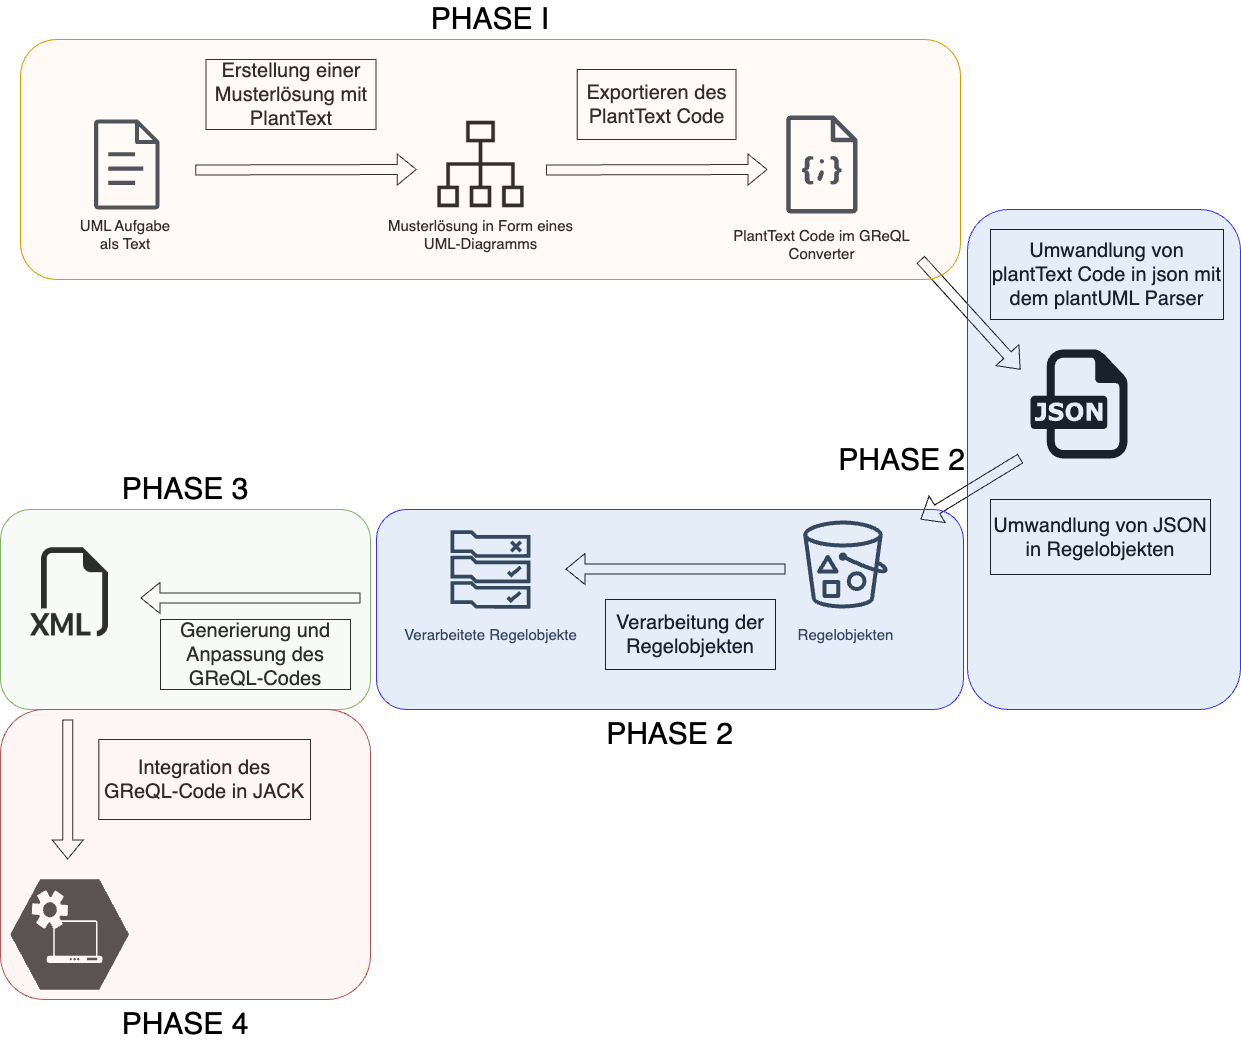
\includegraphics[width=15cm]{images/workflow}
    \caption{repräsentatives Bild des Workflows des GReQL-Converters.}
    \label{fig:workflow}
\end{figure}

\subsubsection{Phase 1: Modellierung einer Musterlösung mit PlantText}

Nachdem der Lehrer eine Übung in Textform erstellt hat, um die Studierenden zu bewerten, muss er die Musterlösung
mithilfe von PlantText modellieren. Dabei müssen bestimmte Kriterien beachtet werden, die in der Dokumentation zur 
Verwendung des GReQL Converters ausführlich beschrieben sind. Diese Kriterien umfassen beispielsweise:

\begin{itemize}
    \item Enums immer mit $<<enum>>$ zu kennzeichnen.
    \item Interfaces immer mit $<<interface>>$ zu annotieren.
    \item Eine spezielle Syntax, die für bestimmte Assoziationen einzuhalten ist.
\end{itemize}

Nachdem der Code für die Musterlösung generiert wurde, kann der Lehrer zur Phase 2 übergehen.


\subsubsection{Phase 2: Verarbeitung der auf dem GReQL Converter erzeugten Regeln}

In der Phase der Regelbearbeitung, die auf die Codegenerierung folgt, hat die Lehrkraft die Aufgabe, den generierten
Code in den GReQL Converter zu übertragen. In dieser Phase entstehen eine Vielzahl von anpassbaren Regeln. Die Anpassung
erfolgt gemäß den spezifischen Bewertungskriterien, die die Lehrkraft verfolgt. Es ist hierbei möglich, Änderungen an
den Regeln vorzunehmen, je nachdem, welche Aspekte der Übung bewertet werden sollen. Weiterhin besteht die Option,
Regeln hinzuzufügen oder zu entfernen. In der Bearbeitung der Regeln ergibt sich auch die Möglichkeit, individuelles
Feedback für jede einzelne Regel hinzuzufügen und die Punktzahl für jede Regel erneut zu justieren.


\subsubsection{Phase 3: Generierung des GReQL-Codes}

Sobald die Phase der Regelbearbeitung (Phase 2) abgeschlossen ist, kann die Lehrkraft den GReQL-Code auf der Plattform
generieren. Dabei orientiert sich die Generierung an den zuvor definierten Regeln. Der generierte GReQL-Code kann,
falls erforderlich, weiterhin angepasst werden.

Dieser Bearbeitungsschritt ist nur dann sinnvoll, wenn der Lehrer bereits über Kenntnisse in GReQL zur Generierung von
Regeln für Klassendiagramme verfügt. Dies ermöglicht es ihm, einige Details des Codes zu verfeinern. Der Zweck des
GReQL Converters ist es, den GReQL-Code zu generieren, der am besten auf die Erwartungen der Lehrkraft eingeht, so dass
dieser Änderungsschritt einfach übersprungen wird. Es ist jedoch möglich, dass dieser Schritt zu Beginn noch notwendig
ist.

\subsubsection{Phase 4: Übertragung des GReQL-Codes auf JACK}

Nach Beendigung der Phase 3 kann die Lehrkraft den generierten GReQL-Code auf die JACK-Plattform übertragen. Dies
erfolgt, nachdem die Übung auf der Plattform erstellt wurde. Anschließend haben die Benutzer die Möglichkeit, ihre
Übungen einzureichen, woraufhin eine Bewertung mit entsprechendem Feedback erfolgt.


Die hier skizzierten Phasen repräsentieren einen essenziellen Schritt in der Umsetzung des im vorherigen Kapitel Ansatzes
zur Bewertung von UML-Diagrammen. Die Dokumentation dieses Prozesses gewährt einen
umfassenden Einblick in die technischen Aspekte des Projekts und erlaubt eine transparente Darstellung des
Implementierungsprozesses.

\section{Einrichtung und Entwicklung des ``GReQL Converter''}